\subsection{Análisis de modelo de onda}
\label{sec:waves_analisys}

Si tomamos el ejemplo de la cuerda, pero ahora en vez de generar un pulso generamos un tren de pulsos como se muestra en la figura \ref{fig:wave_train} sabemos que la onda será transversal y también que las partículas que conforman la cuerda vibran con un movimiento armónico simple. De ahí podemos definir algunas cantidades importantes.

\begin{figure}[ht]
  \centering
  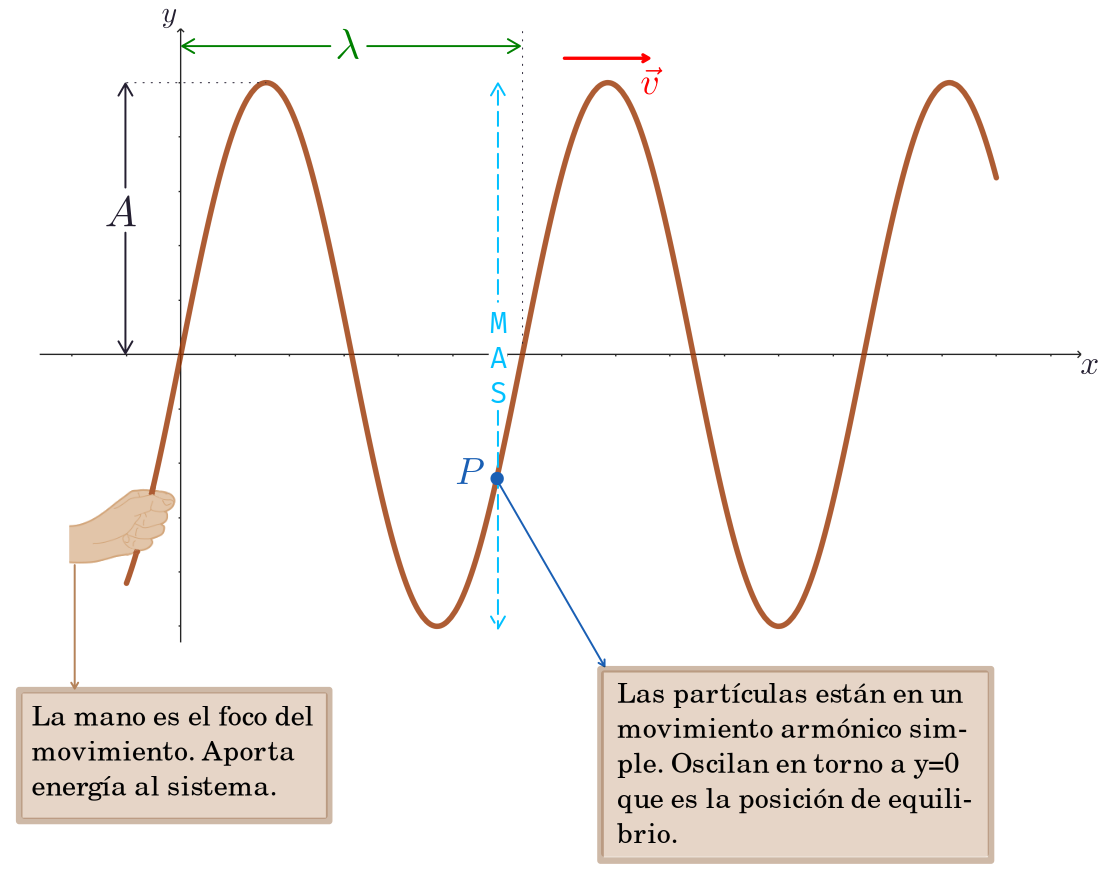
\includegraphics[width=0.8\textwidth]{wave_train.png}
  \caption{Un tren de pulsos que viajan a lo largo de la cuerda.}
  \label{fig:wave_train}
\end{figure}

A continuación te presento las \textit{cantidades físicas básicas} que caracterizan a una onda armónica, junto con su definición, unidad en el SI y su relación con otras magnitudes.

\subsubsection{Cantidades físicas básicas de una onda}
\label{sec:waves_basic_quantities}

\paragraph{Amplitud (\(A\))}

Es el valor máximo que alcanza la magnitud oscilante respecto de su posición de equilibrio.

\begin{itemize}
  \item Unidad: depende del tipo de onda, en el caso de ondas mecánicas su unidad es metros (\(\si{\meter}\)).
  \item Interpretación: indica la intensidad o energía de la onda.
  \item No afecta la velocidad, pero sí la energía transportada.
\end{itemize}

\paragraph{Período (\(T\))}

Es el tiempo que tarda un punto del medio en realizar una oscilación completa. Si vemos la figura \ref{fig:wave_train} el punto \(P\) está en un movimiento armónico simple. Una oscilación completa demora \(T\) segundos, que es un período. 

\begin{itemize}
  \item Unidad: segundos (s).
  \item Relación: inversamente proporcional a la frecuencia: \(T = \frac{1}{f}\)
\end{itemize}

\paragraph{Frecuencia (\(f\))}

Es el número de oscilaciones completas por unidad de tiempo.

\begin{itemize}
  \item Unidad: hertz (Hz), donde \(1\, \text{Hz} = 1\, \text{oscilación/s}\).
  \item Relación: \(f = \frac{1}{T}\)
\end{itemize}

\paragraph{Longitud de onda (\(\lambda\))}

Es la distancia entre dos puntos consecutivos que están en la misma fase (por ejemplo, dos crestas sucesivas). Como se ve en la figura \ref{fig:wave_train} la longitud de onda es la distancia entre dos puntos en fase. 

En una onda mecánica, dos puntos están en fase cuando cumplen las siguientes condiciones:

\begin{enumerate}
  \item Tienen el mismo estado de vibración en el mismo instante, es decir:
    \begin{itemize}
      \item Mismo desplazamiento (posición) respecto a la posición de equilibrio.
      \item Misma velocidad (moviéndose en la misma dirección).
      \item Misma aceleración.
    \end{itemize}
  \item La diferencia de fase entre ellos es un múltiplo entero de \(2\pi\) radianes (o \(0\), \(\pm 2\pi\), \(\pm 4\pi\), etc.). 
  \item La distancia entre ellos es un múltiplo entero de la longitud de onda (\(\lambda\)):
   \[
   \Delta x = n\lambda \quad \text{(con \(n = 0, \pm 1, \pm 2, \dots\))}
   \]
\end{enumerate}

Si la diferencia de fase es \(\pi\) radianes (o un múltiplo impar de \(\pi\)), los puntos están en \textbf{oposición de fase} (máximo alejamiento en vibración). Dos puntos están en fase cuando su separación espacial es un múltiplo entero de \(\lambda\) y su diferencia de fase es \(2\pi n\). Esto implica que oscilan sincronizados.

\begin{itemize}
  \item Unidad: metros (m).
  \item Relación: \(\lambda = \frac{v}{f} = v T\)
\end{itemize}

\paragraph{Velocidad de propagación (\(v\))}

Es la velocidad con que se desplaza el frente de onda (es decir, cómo se propaga la perturbación en el medio).

\begin{itemize}
  \item Unidad: metros por segundo (m/s).
  \item Relación fundamental: la velocidad de propagación de una onda es \(v = \lambda f\)
\end{itemize}

La velocidad de propagación depende del medio en el que se propaga la onda. Por ejemplo, la velocidad de propagación de una onda sonora en el aire es de \(343\, \text{m/s}\) a temperatura ambiente. En la materia Física II se trabaja principalmente con la velociad de propagación en un alambre o cuerda fina. 

La velocidad de propagación de una onda en una cuerda tensa indica con qué rapidez se traslada la perturbación (o energía) a lo largo de la cuerda. Esta velocidad depende exclusivamente de las propiedades físicas del medio, es decir, de la tensión aplicada a la cuerda y de su densidad lineal de masa.

La velocidad \(v\) de propagación de una onda transversal en una cuerda idealmente elástica y tensa se calcula mediante la siguiente fórmula:
\[
v = \sqrt{\frac{T}{\mu}}
\]
donde:
\begin{itemize}
  \item \(T\) es la tensión en la cuerda (en newtons, N),
  \item \(\mu\) es la densidad lineal de masa de la cuerda, es decir, la masa por unidad de longitud (en kg/m).
\end{itemize}

Cuanto mayor es la tensión \(T\) en la cuerda, más rápidamente se propaga la onda. Esto es porque la fuerza que ``restaura'' la cuerda hacia su equilibrio es mayor, lo que permite transmitir la perturbación más eficazmente.

Cuanto mayor es la densidad lineal \(\mu\) (es decir, cuanto más pesada es la cuerda por unidad de longitud), más difícil es acelerar sus partículas, lo que reduce la velocidad de propagación.

A nivel conceptual, se puede entender la fórmula considerando un pequeño elemento de cuerda \(\mu \, \mathrm{d}x\), este pequeño elemento de masa está sometido a fuerzas de tensión desde los extremos. Aplicando la segunda ley de Newton al análisis de estas fuerzas y a la aceleración transversal que experimenta el segmento debido a la curvatura local de la cuerda, se obtiene una ecuación de onda. Esta ecuación predice una velocidad de propagación que resulta ser \(v = \sqrt{T / \mu}\).

\paragraph{Número de onda (\(k\))}

Es una medida del número de ciclos por unidad de longitud, análogo espacial de la frecuencia temporal.

\begin{itemize}
  \item Unidad: radianes por metro (rad/m).
  \item Relación: \(k = \frac{2\pi}{\lambda}\)
\end{itemize}

\paragraph{Frecuencia angular (\(\omega\))}

Es la frecuencia expresada en términos angulares (radianes por segundo).

\begin{itemize}
  \item Unidad: rad/s.
  \item Relación: \(\omega = 2\pi f = \frac{2\pi}{T}\)
\end{itemize}

\paragraph{Fase (\(\vartheta\)) y diferencia de fase}

La fase indica en qué punto del ciclo se encuentra la oscilación. Es el mismo concepto de fase que se encuentra en el movimiento armónico simple. Si no lo recuerdas te recomiendo que revises el capítulo \ref{sec:mas}.

Estas cantidades permiten construir la función de onda general de una onda armónica:
\[
y(x, t) = A \cos(kx - \omega t + \varphi)
\]
La deducción de la ecuación de onda la veremos más adelante, por ahora te recomiendo que simplemente la recuerdes y prestes atención al concepto de fase que no requiere que sepas cómo se deduce.

En esta ecuación la fase \(\vartheta\) (variable theta) es el argumento del coseno, es decir \(\vartheta = kx - \omega t + \varphi\). Esta cantidad no tiene unidades, y se mide en radianes. La fase describe en qué punto del ciclo se encuentra la onda en un lugar y momento dados. Dos puntos de la onda que tengan el mismo valor de fase están en la misma etapa del ciclo: por ejemplo, ambos en una cresta o ambos en un nodo.

La diferencia de fase es la distancia angular (en radianes) entre dos ondas o entre dos puntos de una misma onda. Se denota típicamente como \(\Delta \varphi\) o simplemente \(\delta\). En general hay dos contextos donde se habla de diferencia de fase:
\begin{enumerate}
  \item Entre dos ondas distintas
  \item Entre dos puntos de una misma onda
\end{enumerate}

Veamos el primer caso. Supongamos dos ondas con igual frecuencia y número de onda:
\[
\psi_1(x,t) = A \cos(kx - \omega t) \\
\psi_2(x,t) = A \cos(kx - \omega t + \delta)
\]
Entonces, la diferencia de fase entre ambas es \(\delta\). Esto determina si las ondas están en fase (cuando \(\delta = 0\) o múltiplos de \(2\pi\)) o desfasadas (por ejemplo, \(\delta = \pi\) implica interferencia destructiva).

Para el segundo caso la diferencia de fase entre dos posiciones fijas \(x_1\) y \(x_2\) en un instante dado es:
\[
\Delta \theta = k(x_2 - x_1)
\]
Esto se puede expresar como:
\[
\Delta \theta = \frac{2\pi}{\lambda} (x_2 - x_1)
\]
Por lo tanto, dos puntos separados por una longitud de onda completa tienen una diferencia de fase de \(2\pi\) radianes, es decir, están en fase.

Entonces, resumiendo los conceptos tendríamos:
\begin{itemize}
  \item Si dos ondas están en fase, sus crestas y valles coinciden, y se refuerzan al superponerse (interferencia constructiva).
  \item Si están en oposición de fase ($\Delta \varphi = \pi$), las crestas de una coinciden con los valles de la otra (interferencia destructiva).
  \item En sistemas oscilatorios (como masas o circuitos), la fase también indica el retraso temporal entre dos oscilaciones.
\end{itemize}

\subsubsection{Frente de ondas}

El frente de onda es el lugar geométrico de los puntos del medio que están en la misma fase de oscilación en un instante determinado. En otras palabras, es el conjunto de puntos donde la magnitud de la onda (como el desplazamiento) tiene el mismo valor y evolución temporal dentro del ciclo de la onda.

Por ejemplo, en una onda armónica, todos los puntos de un frente de onda alcanzan sus máximos, mínimos y posiciones de equilibrio al mismo tiempo.

El frente de onda proporciona información fundamental sobre la geometría y el comportamiento de la onda. Entre las principales características que define o influye se encuentran:

\paragraph{1. Dirección de propagación}

El frente de onda es \hl{perpendicular} a la dirección en que la energía y la perturbación se propagan. Por lo tanto, la orientación de los frentes determina la dirección del avance de la onda.

\paragraph{2. Forma de la onda}

La geometría del frente de onda determina la naturaleza de la propagación:
\begin{itemize}
  \item Si los frentes son planos, la onda es plana, lo que implica propagación rectilínea desde una fuente lejana o colimada. Las ondas de luz que provienen del sol pueden ser consideradas planas por ejemplo.
  \item Si los frentes son esféricos, la onda se propaga en todas direcciones desde una fuente puntual. El sonido que proviene de un punto fijo en el aire es un ejemplo de onda esférica.
  \item En medios anisótropos o con obstáculos, los frentes pueden deformarse, generando fenómenos como difracción o focalización.
\end{itemize}

\paragraph{3. Interacción con el medio}

La forma y evolución de los frentes de onda permite estudiar fenómenos como:
\begin{itemize}
  \item \hl{Reflexión}: el frente se repliega sobre sí mismo al encontrar una barrera.
  \item \hl{Refracción}: el frente cambia de dirección y velocidad al pasar a otro medio.
  \item \hl{Difracción}: el frente se curva al atravesar rendijas o bordes.
  \item \hl{Interferencia}: superposición de frentes de onda de diferentes fuentes.
\end{itemize}

Analicemos el caso de una onda que interactua con un medio y es \textbf{reflejada}.

\begin{figure}[ht]
  \centering
  \begin{subfigure}[b]{0.32\textwidth}
      \centering
      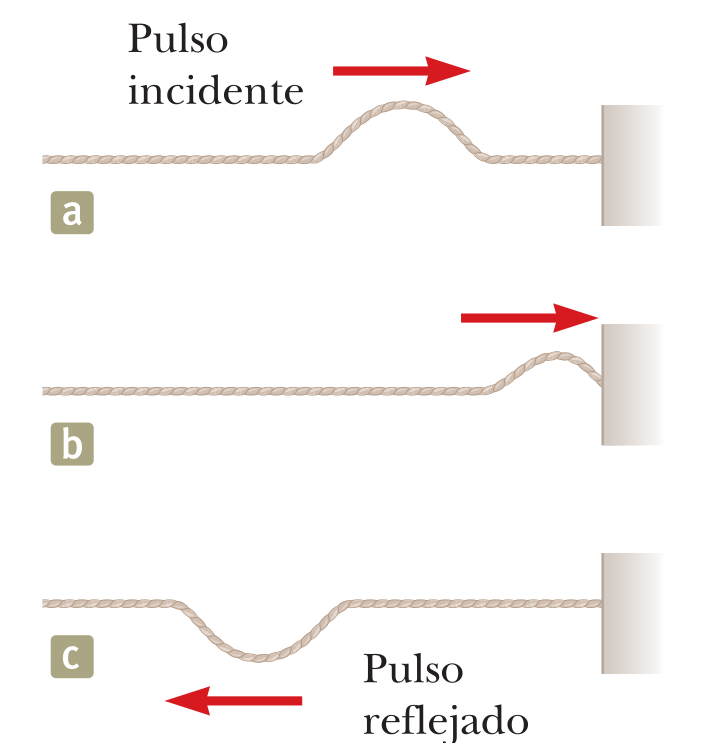
\includegraphics[width=\textwidth]{wave_reflection_fixed.png}
      \caption{El pulso reflejado está invertido, pero su forma no cambia de otra manera.}
      \label{fig:wave_reflection_fixed}
  \end{subfigure}
  \hspace{80pt}
  \begin{subfigure}[b]{0.32\textwidth}
      \centering
      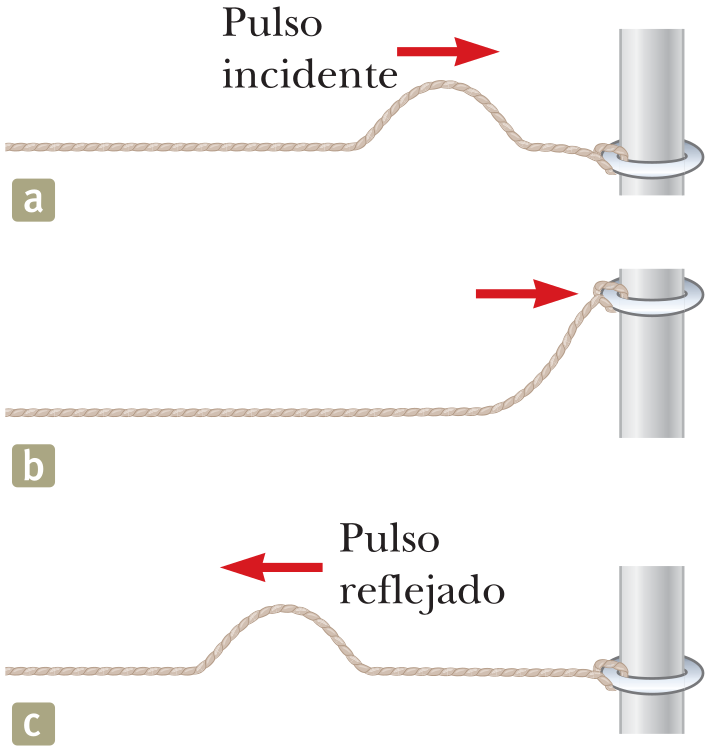
\includegraphics[width=\textwidth]{wave_reflection_loose.png}
      \caption{El pulso reflejado no se invierte, es decir, conserva su dirección original (si iba hacia arriba, vuelve hacia arriba).}
      \label{fig:wave_reflection_loose}
  \end{subfigure}
  \caption{Reflexión de un pulso viajero.}
  \label{fig:wave_reflection}
\end{figure}

\subparagraph{3.1. Reflexión en un extremo fijo (figura \ref{fig:wave_reflection_fixed})}

Cuando la onda llega a un extremo rígidamente fijo, como una cuerda atada a un soporte que no se puede mover, la cuerda genera una fuerza hacia arriba sobre el soporte al llegar el pulso. Por la tercera ley de Newton (acción y reacción), el soporte ejerce una fuerza hacia abajo de igual magnitud sobre la cuerda. Esta fuerza hacia abajo genera una reflexión invertida: el pulso vuelve en sentido contrario, pero con su fase invertida (por ejemplo, si era un pulso hacia arriba, regresa como uno hacia abajo).

\subparagraph{3.2. Reflexión en un extremo libre (figura \ref{fig:wave_reflection_loose})}

Si ahora el extremo de la cuerda es libre de moverse verticalmente, como si estuviera unido a un anillo que puede deslizarse sin fricción, el pulso hace que el anillo se desplace hacia arriba. Luego, la tensión de la cuerda lo jala de regreso hacia abajo, generando un pulso reflejado. En este caso, el pulso reflejado no se invierte, es decir, conserva su dirección original (si iba hacia arriba, vuelve hacia arriba).

\subparagraph{3.3. Reflexión parcial por el cambio de medio}

Esto no solo se aplica para un extremo totalmente fijo o totalmente suelto, también podríamos tener una cuerda pesada atada a una cuerda ligera. En este caso, dependiendo de la configuración, el pulso será parcialmente reflejado y parcialmente transmitido.
\begin{itemize}
  \item Si la onda pasa de un medio menos denso a uno más denso (por ejemplo, de una cuerda ligera a una pesada), el pulso reflejado se invierte.
  \item Si la onda pasa de un medio más denso a uno menos denso (de cuerda pesada a ligera), el pulso reflejado no se invierte.
  \item La densidad está relacionada con la velocidad de propagación: una cuerda ligera permite mayor velocidad que una pesada.
\end{itemize}

\paragraph{4. Velocidad de propagación}

La separación temporal entre frentes consecutivos (por ejemplo, entre dos crestas en el tiempo) y la distancia espacial entre ellos (la longitud de onda) permiten calcular la velocidad de propagación de la onda.